\subsection{Hardware}
\label{sec:hardware}

Our mobile manipulator platform is comprised of various hardware components. 

\paragraph{Robot}
The mobile manipulator is composed of two robots, see Fig.~\ref{fig:hardware}. The moving base is a Clearpath
Boxer, differential drive wheeled-robot. The robotic arm is a Franka Emika
Panda, a serial manipulator with seven degrees of freedom, equipped with torque
sensors in every joint. %, see \cref{fig:layouts}. 
The attached gripper is a
custom 3D-printed suction gripper with two suction cups powered by a industrial
vacuum pump.
\begin{figure}[t]
    \centering    
    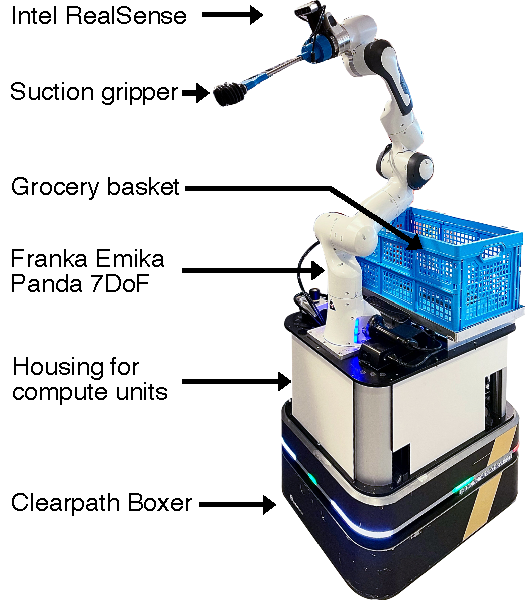
\includegraphics[width=0.65\linewidth]{AlbertHWIntro.pdf}
    \caption{Overview of our robot's hardware.}
    \label{fig:hardware}
\end{figure}


\paragraph{Perception}
The base uses a 270 degree Lidar sensor to localize itself and detect dynamic obstacles and humans in the environment. 
We mounted a Realsense D435 RGBD camera on the wrist
link of the arm and use it to detect products and perform visual servoing during picking.

\paragraph{Compute Units}
We use a total of four compute units to distribute the computational load of individual software components. 
The first compute unit is the Franka Control Unit (FCI) controlling the arm. 
The base's internal compute unit performs
self-localization and collision avoidance for the base.
The central compute
unit is an Intel NUC computer with an Intel i7 10th generation CPU, running all planning components and hosting the user interface for placing orders. 
%Object detection and localization is
%running on an separate laptop mounted on the top of the robot, below the shopping
basket. 
A Dell Alienware laptop mounted on the robot and is equipped with an RTX 3070 TI GPU to run the perception components. %perform
%inference on the detector network and image processing.
Our two computers are running the Robot Operating System (ROS) and communicate via a network switch.
